\documentclass[a4paper]{article}

\addtolength{\hoffset}{-2.25cm}
\addtolength{\textwidth}{4.5cm}
\addtolength{\voffset}{-3.25cm}
\addtolength{\textheight}{5cm}
\setlength{\parskip}{0pt}
\setlength{\parindent}{0in}

%----------------------------------------------------------------------------------------
%	PACKAGES AND OTHER DOCUMENT CONFIGURATIONS
%----------------------------------------------------------------------------------------



\usepackage{blindtext} % Package to generate dummy text
\usepackage{charter} % Use the Charter font
\usepackage[utf8]{inputenc} % Use UTF-8 encoding
\usepackage{microtype} % Slightly tweak font spacing for aesthetics
\usepackage[english]{babel} % Language hyphenation and typographical rules
\usepackage{amsthm, amsmath, amssymb} % Mathematical typesetting
\usepackage{float} % Improved interface for floating objects
\usepackage[final, colorlinks = true,
            linkcolor = black,
            citecolor = black]{hyperref} % For hyperlinks in the PDF
\usepackage{graphicx, multicol} % Enhanced support for graphics
\usepackage{xcolor} % Driver-independent color extensions
\usepackage{marvosym, wasysym} % More symbols
\usepackage{rotating} % Rotation tools
\usepackage{censor} % Facilities for controlling restricted text
\usepackage{listings} % Environment for non-formatted code, !uses style file!
\usepackage{pseudocode} % Environment for specifying algorithms in a natural way
 % Environment for f-structures, !uses style file!
\usepackage{booktabs} % Enhances quality of tables
 % Configuration for b-trees and b+-trees, !uses style file!
\usepackage[backend=biber,style=numeric,
            sorting=nyt]{biblatex} % Complete reimplementation of bibliographic facilities
\addbibresource{ecl.bib}
\usepackage{csquotes} % Context sensitive quotation facilities
\usepackage[yyyymmdd]{datetime} % Uses YEAR-MONTH-DAY format for dates
\renewcommand{\dateseparator}{-} % Sets dateseparator to '-'
\usepackage{fancyhdr} % Headers and footers
\pagestyle{fancy} % All pages have headers and footers
\fancyhead{}\renewcommand{\headrulewidth}{0pt} % Blank out the default header
\fancyfoot[L]{} % Custom footer text
\fancyfoot[C]{} % Custom footer text
\fancyfoot[R]{\thepage} % Custom footer text
\newcommand{\note}[1]{\marginpar{\scriptsize \textcolor{red}{#1}}} % Enables comments in red on margin
\usepackage{mathtools}
\usepackage{amsmath}
\DeclarePairedDelimiter\abs{\lvert}{\rvert}%
\usepackage{cancel}
\usepackage{minted}
\usepackage{float}
\usepackage{enumitem}


\usepackage{tikz-qtree} % Easy tree drawing tool

\usepackage{tikz}
%\usetikzlibrary{shapes,arrows,positioning}
\usetikzlibrary{automata,arrows,positioning,calc}

%-------------------------------

%----------------------------------------------------------------------------------------


%-------------------------------
%	ENVIRONMENT SECTION
%-------------------------------
\pagestyle{fancy}
\usepackage{mdframed}


\newenvironment{problem}[2][Problema]
    { \begin{mdframed}[backgroundcolor=gray!20] \textbf{#1 #2} \\}
    {  \end{mdframed}}

% Define solution environment
\newenvironment{solution}
    {\textit{Solución}}
    {}


%-------------------------------------------------------------------------------------------
%	CUSTOM COMMANDS
%-------------------------------
\newcommand{\gaussian}{\frac{1}{\sigma\sqrt{2\pi}}\exp\left(- \frac{(x-\mu)^2}{2\sigma^2}\right)}
\newcommand{\R}{\mathbb R}

\def\inline{\lstinline[basicstyle=\ttfamily,keywordstyle={}]}


\begin{document}


%-------------------------------
%	TITLE SECTION
%-------------------------------

\fancyhead[C]{}
\hrule \medskip % Upper rule
\begin{minipage}{0.295\textwidth}
\raggedright
\footnotesize
Francisco Javier Sáez Maldonado \hfill\\
77448344F \hfill\\
franciscojavier.saez@estudiante.uam.es
\end{minipage}
\begin{minipage}{0.4\textwidth}
\centering
\large
Examen tiempo continuo\\
\normalsize
Procesos Estocáscicos\\
\end{minipage}
\begin{minipage}{0.295\textwidth}
\raggedleft
\today\hfill\\
\end{minipage}
\medskip\hrule
\bigskip

%-------------------------------
%	CONTENTS
% -------------------------------


\section*{Ejercicio 1}

\subsection*{Enunciado}

Consideremos una sede en red (website) compuesta por tres páginas cuyas etiquetas son $P_{1}, P_{2}, P_{3}$ respectivamente. Para identificar usuarios con un comportamiento atípico supondremos que el patrón de navegación sigue una cadena de Markov en tiempo continuo. Con el fin estimar los parámetros del modelo hemos recopilado datos de navegación para un grupo representativo de usuarios. Los datos han sido registrados el mismo día de la semana y a la misma hora, de forma que podamos asumir que los parámetros del modelo son constantes con el tiempo.\\

Los resultados de las mediciones son los siguientes:


\begin{itemize}
  \item En promedio, los usuarios pasan $2$ minutos en $P_{1}$, 30 segundos en $P_{2}$ y $1$ minuto en $P_{3}$.

  \item Las transitciones entre páginas del sitio en red tienen las siguientes probabilidades

  \begin{table}[H]
    \centering
\begin{tabular}{llll}
Estado inicial / final & $P_1$   & $P_2$   & $P_3$   \\
$P_1$                  & $\star$ & $0.2$   & $0.8$   \\
$P_2$                  & $0.3$   & $\star$ & $0.7$   \\
$P_3$                  & $0.6$   & $0.4$   & $\star$
\end{tabular}
\end{table}
\end{itemize}

Se pide:

\begin{enumerate}[label = (\alph*)]
  \item Dibuja el diagrama de transiciones de la cadena de Markov. Etiqueta las transiciones con la probabilidad correspondiente.

  \item Escribe la matriz de transciciones para el proceso de saltos subyacente (\emph{jump process}).




\end{enumerate}


\subsection*{Solución}

Consideraremos los tiempos en minutos, es decir, $30$ segundos es $0.5$ minutos.\\

Además comentamos lo siguiente: Se nos dice que, en promedio, los usuarios pasan cierto tiempo en cada una de las web. Es decir, se nos está indicando el \emph{holding time} de este proceso de saltos. Sabemos que este \emph{holding time} se distribuye según una distribución exponencial de parámetro $\lambda_{i}$. Además, sabemos que la media de una distribución exponencial de parámetro $\lambda$ es $\frac{1}{\lambda}$. Es decir, la información que se nos está dando son los $\frac{1}{\lambda_{i}}$. Por ello, cambiamos estos parámetros a
\[
\lambda_{1} = \frac{1}{2}, \quad \lambda_{2} = 2, \quad \lambda_{3} = 1
\]

Procedemos a resolver el ejercicio.

\begin{enumerate}[label=(\alph*)]
  \item Dibujamos primero el diagrama de transiciones de la cadena de Markov. El resultado es el siguiente
        \begin{center}
	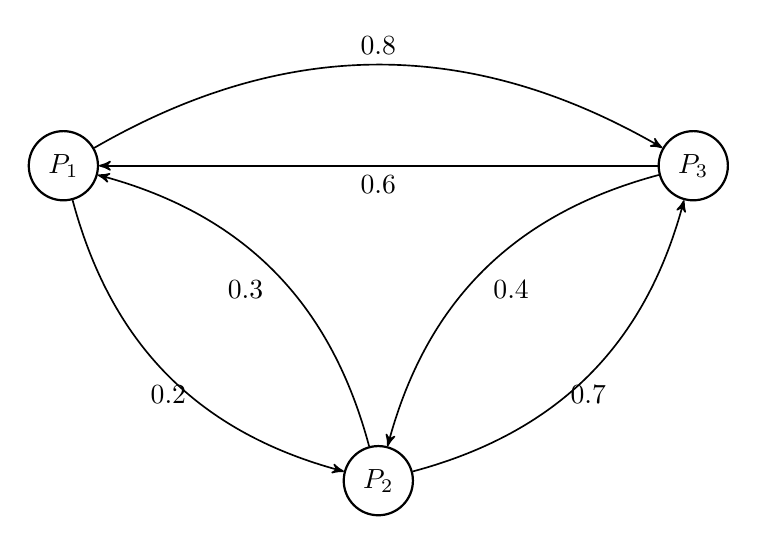
\begin{tikzpicture}[->, >=stealth', auto, semithick, node distance=3cm]
	\tikzstyle{every state}=[fill=white,draw=black,thick,text=black,scale=1]
	\node[state]  at (-4,3)  (A)                     {$P_1$};
	\node[state]    (B) at(0,-1)   {$P_2$};
	\node[state]    (C)at(4,3)   {$P_3$};
	\path
	(A) edge[bend right, below] node{$0.2$} (B)
	(A) edge[bend left, above] node{$0.8$}(C)

	(B) edge[bend right] node{$0.3$} (A)
	(B) edge[bend right, below] node{$0.7$} (C)

	(C) edge node{$0.6$} (A)
	(C) edge[bend right] node{$0.4$} (B);
	\end{tikzpicture}
  \end{center}


\item Escribimos a partir de esta cadena de Markov la matriz de transiciones para el proceso de saltos

\[
         \mathbf{ \tilde P }  =
        \begin{pmatrix}
          0 & 0.2 & 0.8 \\
          0.3 & 0 & 0.7 \\
          0.6 & 0.4 & 0
        \end{pmatrix}
\]

\item Vamos a derivar la distribución estacionaria para este proceso de saltos. Para ello, debemos encontrar aquel vector propio que tiene valor propio $1$, es decir, debemos encontrar

\[
\begin{pmatrix}\tilde \pi_1 & \tilde \pi_2 & \tilde \pi_3 \end{pmatrix}
        \begin{pmatrix}
          0 & 0.2 & 0.8 \\
          0.3 & 0 & 0.7 \\
          0.6 & 0.4 & 0
        \end{pmatrix} = \begin{pmatrix}\tilde \pi_1 & \tilde \pi_2 & \tilde \pi_3 \end{pmatrix}
\]
Tenemos que resolver por tanto el sistema de ecuaciones que obtenemos.

        \[
        \begin{cases}
          0.3 \tilde \pi_{2} + 0.6 \tilde \pi_{3} = \tilde \pi_{1}\\
          0.2 \tilde \pi_{1} + 0.4 \tilde \pi_{3} = \tilde \pi_{2}\\
          0.8 \tilde \pi_{1} + 0.7 \tilde \pi_{2} = \tilde \pi_{3}
          \end{cases}
        \]
        Y usar la condicición extra de que $\tilde \pi_1 + \tilde \pi_2 + \tilde \pi_3  = 1$. Resolviendo este sistema (podemos encontrar la solución \href{https://www.wolframalpha.com/input/?i=systems+of+equations+calculator&assumption=%7B%22F%22%2C+%22SolveSystemOf4EquationsCalculator%22%2C+%22equation1%22%7D+-%3E%22x+%3D+0.3*y+%2B+0.6*z%22&assumption=%22FSelect%22+-%3E+%7B%7B%22SolveSystemOf4EquationsCalculator%22%7D%7D&assumption=%7B%22F%22%2C+%22SolveSystemOf4EquationsCalculator%22%2C+%22equation2%22%7D+-%3E%22y+%3D+0.2*x+%2B+0.4*z%22&assumption=%7B%22F%22%2C+%22SolveSystemOf4EquationsCalculator%22%2C+%22equation3%22%7D+-%3E%22z+%3D+0.8*x+%2B+0.7*y%22&assumption=%7B%22F%22%2C+%22SolveSystemOf4EquationsCalculator%22%2C+%22equation4%22%7D+-%3E%22x+%2B+y+%2B+z+%3D+1%22}{aquí}) obtenemos que la solución es
        \[
        \mathbf{\tilde \pi} = \begin{pmatrix}\tilde \pi_1 & \tilde \pi_2 & \tilde \pi_3 \end{pmatrix} = \begin{pmatrix}\frac{36}{109} & \frac{26}{109} & \frac{47}{109} \end{pmatrix}
        \]
        y esta es la distribución estacionaria del proceso de saltos subyacente.

  \item Usando esta distribución estacionaria, podemos derivar la distribución estacionaria de nuestra CTMC inicial.

        Sabemos que, asumiendo que $0 < \sum_{k \in S} \frac{\tilde \pi_{k}}{\lambda_{k}} < \infty$, entonces
        \begin{equation}\label{stationary:ctmc}
\pi_{j} = \lim_{t \to \infty} \mathbb P(X(t) = j \ | \ X(0) = i) = \frac{ \frac{\tilde \pi_{j}}{\lambda_{j}} }{\sum_{k \in S}\frac{\tilde \pi_{k}}{\lambda_{k}}}.
        \end{equation}
        Podemos aplicar directamente esto para obtener:
        \[
\pi_1 \propto \frac{\tilde \pi_1}{\lambda_1} = \frac{72}{109} \\
\]
\[
\pi_2 \propto \frac{\tilde \pi_2}{\lambda_2} = \frac{26}{218} = \frac{13}{109}  \\
\]
\[
\pi_3 \propto \frac{\tilde \pi_3}{\lambda_3} = \frac{47}{109} \\
        \]
        Debemos volver a usar la condición de normalización para $\pi_1 + \pi_2 + \pi_3 = 1$, para obtener la distribución estacionaria de la CTMC:
        \[
        \mathbf{\pi} = \begin{pmatrix} \pi_1 &  \pi_2 &  \pi_3 \end{pmatrix}  =
        \begin{pmatrix}
          \frac{72}{132} & \frac{13}{132}&\frac{47}{132}
        \end{pmatrix}
        \]



  \item Tenemos que generar el generador infinitesimal $\mathbf G$. Para ello, sabemos que (en el caso concreto de una CTMC) este está dado por:
        \[
g_{ij} =
\begin{cases}
\lambda_i p_{ij} & i \neq j\\
-\lambda _i & i = j
\end{cases}.
        \]
        Por lo que, aplicado a nuestro caso, obtenemos:
        \[
        \mathbf{G} = \begin{pmatrix}
          -0.5 & 0.1 & 0.4 \\
          0.6 & -2 & 1.4 \\
          0.6 & 0.4 & -1
        \end{pmatrix}
        \]

  \item A continuación, queremos comprobar que hemos encontrado la distribución estacionaria del proceso correctamente. Para ello, vamos a derivar la distribución estacionaria del proceso usando el generador infinitesimal y la compararemos.

        Sabemos que en una CTMC con distribución estacionaria $\pi$ y generador infinitesimal $G$,  se cumple que
        \[
        \pi^{T} \mathbf{G} = 0.
        \]
        Podemos aplicar esto a nuestro problema:
        \[
        \pi^{T} \mathbf G = \begin{pmatrix} \pi_{1} & \pi_{2} & \pi_{3} \end{pmatrix}    \begin{pmatrix}
          -0.5 & 0.1 & 0.4 \\
          0.6 & -2 & 1.4 \\
          0.6 & 0.4 & -1
        \end{pmatrix} = 0
        \Longleftrightarrow
        \begin{cases}
          -0.5 \pi_{1} + 0.6 \pi_{2} + 0.6\pi_{3} = 0 \\
          0.1 \pi_{1} - 2\pi_{2}+ 0.4 \pi_{3} = 0\\
          0.4 \pi_{1} + 1.4 \pi_{2} - \pi_{3} = 0
          \end{cases}
        \]
        Si resolvemos este sistema (podemos encontrar la solución \href{https://www.wolframalpha.com/input/?i=systems+of+equations+calculator&assumption=%7B%22F%22%2C+%22SolveSystemOf4EquationsCalculator%22%2C+%22equation1%22%7D+-%3E%22+-0.5*x+%2B++0.6*y+%2B0.6*z+%3D+0%22&assumption=%22FSelect%22+-%3E+%7B%7B%22SolveSystemOf4EquationsCalculator%22%7D%7D&assumption=%7B%22F%22%2C+%22SolveSystemOf4EquationsCalculator%22%2C+%22equation2%22%7D+-%3E%220.1*x+-+2*y+%2B+0.4*z+%3D+0%22&assumption=%7B%22F%22%2C+%22SolveSystemOf4EquationsCalculator%22%2C+%22equation3%22%7D+-%3E%220.4*x+%2B+1.4*y+-+z+%3D+0%22&assumption=%7B%22F%22%2C+%22SolveSystemOf4EquationsCalculator%22%2C+%22equation4%22%7D+-%3E%22x+%2B+y+%2B+z+%3D+1%22}{aquí}), obtenemos que
        \[
        \pi = \begin{pmatrix} \pi_{1} & \pi_{2} & \pi_{3} \end{pmatrix} = \begin{pmatrix} \frac{72}{132} & \frac{13}{132} & \frac{47}{132} \end{pmatrix},
        \]
        que es el mismo resultado que obtuvimos anteriormente, como podíamos esperar. Con esto lo que podemos decir es que podemos obtener la distribución estacionaria de nuestra CTMC a través de, o bien la distribución estacionaria del proceso de saltos asociado y los $\lambda_{i}$ de este proceso de saltos, o bien usando el generador infinitesimal de nuestra CTMC.

  \item Este apartado está resuelto en el cuaderno de jupyter.
  \item Este apartado también se puede encontrar en el cuaderno de jupyter.
  \item Las distribución estacionaria de la cadena de Markov en tiempo discreto (que puede ser vista como quedarnos únicamente con los saltos olvidándonos del tiempo que pasa en cada estado \emph{holding time}, es decir, como los saltos del proceso de saltos), \textbf{no tiene por qué coincidir en general} con la distribución estacionaria de la CTMC aunque tengan el mismo diagrama de transición.

        Es precisamente por el hecho de que el \emph{holding time} en cada uno de los estados sea diferente, lo que hace que la probabilidad de estar en un estado en cada momento de tiempo no dependa únicamente de la probabilidad de ir de un estado a otro, sino también del tiempo.

        Para que estas dos distribuciones \textbf{coincidiesen}, deberíamos tener que la media de tiempo de salto (es decir, el parámetro $\lambda_{i}$) fuese el mismo en todos los casos. En la Ecuación \eqref{stationary:ctmc}, hemos visto que podemos establecer una relación entre $\tilde \pi$ y $\pi$. Usando esta relación, comprobamos que podemos establecer una condición suficiente para que estas distribuciones coincidan. Si $\lambda_{i} = \lambda_{j}$ para todo $i \neq j$, se tiene entonces que la ecuación \eqref{stationary:ctmc} se convierte en
        \[
        \pi_{j} = \lim_{t \to \infty} \mathbb P(X(t) = j \ | \ X(0) = i) = \frac{ \frac{\tilde \pi_{j}}{\lambda_{j}}}{\frac{1}{\lambda_{j}} \sum_{i \in S}\tilde \pi_{i}} = \frac{\tilde \pi_{j}}{1} = \tilde \pi_{j},
        \]

        con lo que tendríamos que la distribución estacionaria de la CTMC y de la cadena de markov en tiempo discreto coinciden, como queríamos buscar.


  \item Queremos ahora generalizar el modelo actual para incluir usuarios que acceden desde páginas externas o abandonen/entren al sitio web.

        Para esto, lo primero que podemos pensar es en añadir un \textbf{nuevo estado} al sistema que mantenga a las personas que están fuera del sistema (en cualquier sitio, tanto fuera de internet como dentro pero en diferentes páginas web), y que tengan una probabilidad de entrar y de salir del sistema en cada salto. Se puede asumir que,

        \begin{itemize}
          \item A priori, la probabilidad de entrar a cada una de las páginas desde fuera del sistema es la misma para todas las páginas del sistema. Podemos llamarla $P_{in}$.
                \item De igual modo, la probabilidad de salir del sistema estando en cualquiera de las páginas es la misma. Podemos llamarla $P_{out}$.
        \end{itemize}

        Podemos visualizar el modelo haciendo su diagrama de transiciones. Para esto, debemos modificar el anterior, sabiendo que además ahora las probabilidades de ir de una página web a otra cambian, pues tenemos ahora un nuevo estado al que también hay probabilidad de ir desde cada página web. El diagrama resultante es el siguiente.
          \begin{center}
	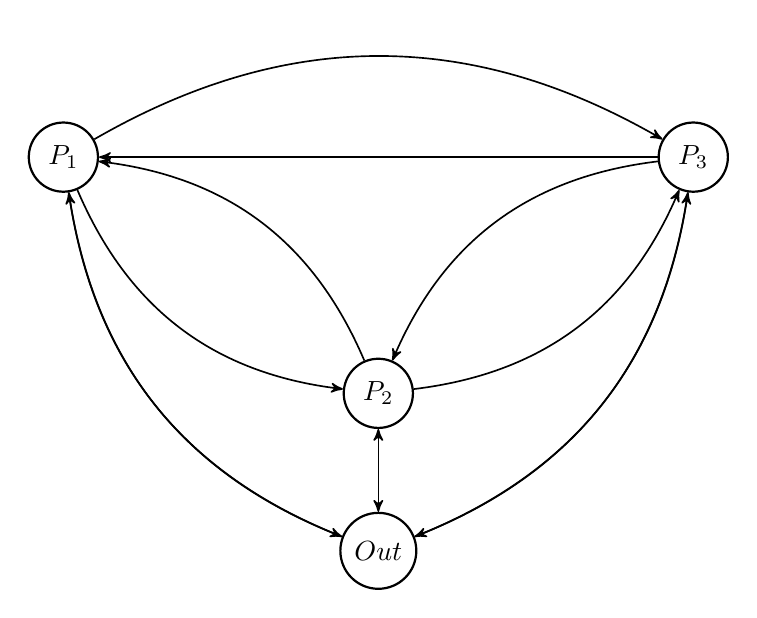
\begin{tikzpicture}[->, >=stealth', auto, semithick, node distance=3cm]
	\tikzstyle{every state}=[fill=white,draw=black,thick,text=black,scale=1]
	\node[state]  at (-4,3)  (A)                     {$P_1$};
	\node[state]    (B) at(0,0)   {$P_2$};
	\node[state]    (C) at (4,3)   {$P_3$};
    \node[state] (F) at (0,-2) {$Out$};
	\path
	(A) edge[bend right]  (B)
	(A) edge[bend left] (C)

	(B) edge[bend right]  (A)
	(B) edge[bend right]  (C)

	(C) edge  (A)
	(C) edge [bend right] (B)

    (A) edge [bend right]  (F)
    (F) edge [bend left] (A)

    (B) edge (F)
    (F) edge (B)

    (C) edge [bend left] (F)
    (F) edge [bend right] (C);

	\end{tikzpicture}
  \end{center}

        Según este sencillo nuevo modelo, podemos trabajar con las probabilidades de salir $P_{out}$ y entrar $P_{in}$ al sistema para ver en qué condiciones el modelo alcanzaría un estado estacionario. Tenemos los siguientes casos:

        \begin{itemize}
          \item Si $P_{in} > P_{out}$, entonces tendremos que más usuarios entran al sistema de los que salen, por tanto con el tiempo todos los usuarios acabarán estando dentro del sistema. En este momento, el nuevo sistema tendrá un estado estacionario \textbf{si, y sólamente si}, el subsistema formado por las páginas web tiene un estado estacionario. En el caso de nuestro subsistema anterior, ya hemos visto que no tiene un estado estacionario, pero esto podría cambiar si cambiásemos las probabilidades de los estados (como hemos dicho que tenemos que hacer al añadir una probabilidad de entrada/salida al sistema).

          \item Si $P_{out} > P_{in}$, entonces todos los usuarios acabarán saliendo del sistema, por lo que tendremos que el estado \emph{Out} es un estado estacionario del sistema.

                \item Si $P_{out} = P_{in}$, el análisis debería ser mucho más extenso. En este caso, deberíamos tener en cuenta si hay estados estacionarios o absorbentes dentro de cada uno de los subsistemas (considerando como subsistema dentro/fuera), y deberíamos tener también en cuenta si el \emph{holding time} de ir de dentro del subsistema a fuera del subsistema es el mismo o no es el mismo, pues si el holding time (es decir, el parámetro $\lambda$ de la distribución del proceso de saltos de entrada/salida)... En definitiva, tendríamos que hacer ciertas hipótesis más concretas sobre probabilidades y holding times y realizar de nuevo el estudio que hemos hecho hasta ahora en los apartados anteriores del problema.
        \end{itemize}

        Además de esto, las hipótesis iniciales del problema son también \textbf{bastante restrictivas}. Por ejemplo, estamos asumiendo que la población (y, por tanto el número de usuarios) es constante, cuando en realidad posiblemente deberíamos utilizar un modelo de cadena de CTMC \emph{birth-death} para modelar cómo se mueve la población. Podríamos ponernos aún más exquisitos y modelar que las probabilidades de entrada al sistema web o a la página son diferentes según los grupos de edad, por eso hemos propuesto un modelo preliminar sencillo, porque estudiar todos los factores que podrían afectar al sistema completo es un problema de una complejidad muy elevada.
\end{enumerate}

\section*{Ejercicio 2 - Modelo de Vasicek}

\subsection*{Enunciado}

En el modelo de Vasicek se realiza la suposición de que la curva que describe la evolución del tipo de interés a corto plazo con el tiempo $r(t)$ es una realización de un proceso de Ornstein-Uhlenbeck. La ecuación diferencial estocástica para este proceso es

\begin{equation}\label{sde}
  d r(t) = - \alpha(r(t) - r_{\infty}) + \sigma dW(t), \quad r(s) \perp dW(t), \ \forall s \leq t
\end{equation}
donde $\alpha > 0$ es la tasa de inversión a la media, $r_{\infty}$ es el tipo de interés a largo plazo y $\sigma > 0$ la volatilidad instantánea.

Este proceso tiene las siguientes propiedades:
\begin{itemize}
  \item Es estacionario
  \item Presenta reversión a la media
\end{itemize}

La solución de esta ecuación diferencial estocástica para $t \geq t_{0}$ a partir de la condición inicial $r(t_{0}) = r_{0}$ es
\begin{equation}\label{sol:sde}
r(t) = r_{\infty} + (r_{0} - r_{\infty})e^{-\alpha(t-t_{0})} + \sigma \sqrt{\frac{1 - e^{-2\alpha(t-t_{0})}}{2\alpha}}Z, \quad Z \sim N(0,1)
\end{equation}

\subsection*{Solución}

\begin{enumerate}[label=(\alph*)]
  \item \label{2:a} Queremos calcular primero las expresiones de $\mathbb E[r(t)|r(t_{0}) = r_{0}]$ y $Cov[r(t),r(t') \ | \ r(t_{0})= r_{0}]$, usando para ello la Ecuación \eqref{sol:sde}. Comenzamos con la esperanza. En este caso, basta utilizar que el operador esperanza es lineal y que la esperanza de una constante es la propia constante, para obtener lo siguiente:

        \begin{align*}
         \mathbb E[r(t)|r(t_{0}) = r_{0}] & = \mathbb E\left[ r_{\infty} + (r_{0} - r_{\infty})e^{-\alpha(t-t_{0})} + \sigma \sqrt{\frac{1 - e^{-2\alpha(t-t_{0})}}{2\alpha}}Z\right] \\
                         & =  r_{\infty} + (r_{0} - r_{\infty})e^{-\alpha(t-t_{0})} + \sigma \sqrt{\frac{1 - e^{-2\alpha(t-t_{0})}}{2\alpha}} \underbrace{\mathbb E[Z]}_{0} \\
          & = r_{\infty} + (r_{0} - r_{\infty})e^{-\alpha(t-t_{0})}
        \end{align*}

        Vamos ahora con la covarianza. Usamos la bilinealidad de la covarianza que, en general, se escribe como
        \[
        Cov(aX+bY, cW + dV) = acCov(X,W) + adCov(X,V) + bcCov(Y,W) + bdCov(Y,V).
        \]
        Aplicando esto a nuestro caso, tenemos que los términos que sean constantes desaparecerán pues la covarianza con una constante es cero. Por tanto,
        \begin{align*}
          Cov[r(t), r(t')|r(t_{0}) = r_{0}] & = \sigma^{2}\sqrt{\frac{1- e^{-2\alpha (t-t_{0})}}{2\alpha}}\sqrt{\frac{1- e^{-2\alpha (t'-t_{0})}}{2\alpha}}\underbrace{Cov\left[Z,Z\right]}_{1} \\
          & =  \sigma^{2}\sqrt{\frac{1- e^{-2\alpha (t-t_{0})}}{2\alpha}}\sqrt{\frac{1- e^{-2\alpha (t'-t_{0})}}{2\alpha}}
        \end{align*}

  \item \label{2:c} Ahora, supondremos que $r_{\infty}$ y $r_{0}$ son del mismo orden de magnitud. Queremos ver en qué escala de tiempo (es decir, a partir de qué $t$) se alcanza el estado estacionario para este proceso. Vemos que la expresión del estado estacionario de la solución $r(t)$
        \[
        \lim_{t \to \infty} r(t) = \lim_{t \to \infty}  r_{\infty} + (r_{0} - r_{\infty})e^{-\alpha(t-t_{0})} + \sigma \sqrt{\frac{1 - e^{-2\alpha(t-t_{0})}}{2\alpha}}Z = r_{\infty} +  \sigma \sqrt{\frac{1}{2\alpha}}Z.
        \]

        Vemos que este límite existe debido a que la \textbf{exponencial} negativa tiende a cero. Además, la dependencia de que este límite existe es únicamente de esta función exponencial, por lo que podemos decir que la escala de tiempo con la que se alcanza el estado estacionario es \textbf{exponencial}.



        Consideraremos ahora que $1$ y $1+eps$ con $eps \approx 10^{-16}$ son idénticos, y queremos ver cuánto tiempo tarda la diferencia entre el valor de $r(t)$ y el límite obtenido es menor que este $10^{-16}$, pudiendo afirmar así que estamos en el estado estacionario. Para ello, tenemos que encontrar el $t$ tal que:
        \[
        \abs{\lim_{t\to \infty}r(t) - r(t)} \leq 10^{-16}.
        \]
        Para esto, vemos que
        \begin{align*}
          \left(\lim_{t\to \infty}r(t)\right) - r(t) & = r_{\infty}  + \sigma \sqrt{\frac{1}{2\alpha}}Z - \left( r_{\infty} + (r_{0} - r_{\infty})e^{-\alpha(t-t_{0})} + \sigma \sqrt{\frac{1 - e^{-2\alpha(t-t_{0})}}{2\alpha}}Z \right)\\
                                                     & = \sigma \sqrt{\frac{1}{2\alpha}}Z\left(1 - \sqrt{1 - e^{-2\alpha(t-t_{0})}}\right) - (r_{0} - r_{\infty})e^{-\alpha(t-t_{0})}\\
          & = h(t),
        \end{align*}
        donde, en la última línea hemos decidido llamar a esa expresión $h(t)$. Esto lo hacemos porque, usando $h(t)$, lo que queremos buscar es el $t$ tal que
        \[
        \abs{h(t)} \leq 10^{-16},
        \]
        y este sería el tiempo necesario para considerar que, numéricamente, el proceso está en el estado estacionario.

  \item  Ahora queremos usar las expresiones obtenidas en el apartado \label{2:a} para derivar las funciones de media y covarianzas en el estado estacionario: $\mathbb E[r(t)]$ y $Cov[r(t), r(t')]$. Podemos suponer que, como estamos en el estado estacionario, ha pasado el suficiente tiempo para que el proceso converga a este estado, así que podemos tomar la esperanza en el límite cuando el tiempo tiende a infinito, y usar así la expresión que hemos calculado en el apartado anterior.

        \begin{align*}
          \lim_{t\to \infty} \mathbb E [r(t)] & = \mathbb E \left[ \lim_{t \to \infty} r(t)\right] \\
                                              & = E \left[r_{\infty}  + \sigma \sqrt{\frac{1}{2\alpha}}Z\right]\\
          & = r_{\infty}
        \end{align*}
        Para la covarianza, podemos también suponer que, como ha pasado el suficiente tiempo y estamos en el estado estacionario, calcular la covarianza en el mismo tiempo $t$ (es decir, la varianza de $r(t)$ en ese tiempo $t$) a partir del cual habíamos dicho en el apartado anterior que teníamos el proceso (numéricamente) en el estado estacionario.

        \begin{align*}
          \lim_{t\to \infty} Cov[r(t), r(t)] & = \lim_{t \to \infty} Var[r(t)] \\
         & = \lim_{t \to \infty} \sigma^{2}\sqrt{\frac{1- e^{-2\alpha (t-t_{0})}}{2\alpha}}\sqrt{\frac{1- e^{-2\alpha (t'-t_{0})}}{2\alpha}}\\
          & =  \sigma^{2} \sqrt{ \frac{1}{2\alpha} }
        \end{align*}

  \item \label{2:d} Ahora, queremos hallar la expresión de $ \mathbb P(t,r(t) \ | \ t_{0},r_{0})$. Para ello, tenemos que ver que esto sigue una distribución normal de ciertos parámetros pues, al estar condicionando a una condición inicial $r_{0}$ y un tiempo inicial $t_{0}$, lo que está ocurriendo es que nuestra función $r(t)$ se convierte en un proceso de Wiener al que se el parámetro $t$ que tenemos habitualmente, se le ha realizado una transformación para que no sea un Wiener \emph{estándar} (que consideramos como $W(t) \sim N(0,\sqrt{t})$). Es por ello que, usando las expresiones obtenidas en el apartado \ref{2:a}, podemos decir que :
        \[
        \mathbb P(t,r(t) \ | \ t_{0}, r_{0}) \sim N\left(r_{\infty} + (r_{0} - r_{\infty})e^{-\alpha(t-t_{0})}, \sigma^{2} \frac{1 - e^{-2\alpha (t-t_{0})}}{2\alpha}\right)
        \]

  \item \label{2:e} Queremos hallar también las expresiones de esto en el estado estacionario. Para esto,podemos argumentar del mismo modo que en el apartado anterior, pero sabiendo que ahora el $t$ es suficientemente grande para estar en el estado estacionario del proceso. Es decir, podemos considerar el límite cuando $t \to \infty$. Así, podemos simplemente afirmar de nuevo que nuestro proceso sigue una distribución normal (al igual que la seguía en el apartado anterior), y usar como nuevos parámetros de esta distribución normal los límites que hemos calculado en el apartado \ref{2:c}. Es por ello que afirmamos que, en el estado estacionario,
        \[
        P(t,r(t)\ | \ t_{0}, r_{0}) \sim N\left(r_{\infty}, \sigma^{2}\sqrt{\frac{1}{2\alpha}}\right)
        \]

  \item Nuestro objetivo en este apartado es encontrar dos límites. Empezamos con el primero, que es:
        \[
        \lim_{t \to 0} \mathbb P(t,r(t) \ | \ t_{0}, r_{0}).
        \]
        En este caso, podemos usar que en el apartado \ref{2:d} hemos hallado qué distribución sigue esta probabilidad, para decir que el límite cuando $t \to 0$ de esta probabilidad será el límite que tenga la función de densidad de una normal de media y varianza halladas en ese apartado \ref{2:d}. Al tomar este límite, obtendremos que
        \[
        \lim_{t\to 0} P(t,r(t) \ | \ t_{0}, r_{0}) \sim \lim_{t \to 0}  N\left(r_{\infty} + (r_{0} - r_{\infty})e^{-\alpha(t-t_{0})}, \sigma^{2} \frac{1 - e^{-2\alpha (t-t_{0})}}{2\alpha}\right) = N\left(r_{0}, 0\right)
        \]

        El segundo límite es justamente lo que ya habíamos calculado anteriormente en el apartado \ref{2:e}. En el caso anterior, podríamos no haber considerado el límite y haber supuesto simplemente que el $t$ que estábamos usando era suficientemente grande, pero hemos decidido tomar ese límite. Es por ello que, en este caso, repetimos la solución teniendo que

          \[
        \lim_{t\to \infty} P(t,r(t)\ | \ t_{0}, r_{0}) \sim N\left(r_{\infty}, \sigma^{2}\sqrt{\frac{1}{2\alpha}}\right)
        \]
  \item Resuelto en el cuaderno de jupyter.

  \item Resuelto en el cuaderno de jupyter.

  \item Resuelto en el cuaderno de jupyter.

  \item Resuelto en el cuaderno de jupyter.
  \item Resuelto en el cuaderno de jupyter.
  \item Resuelto en el cuaderno de jupyter.

\end{enumerate}
\end{document}
